
\documentclass[a4paper,11pt]{article}
\usepackage[a4paper, margin=8em]{geometry}

% usa i pacchetti per la scrittura in italiano
\usepackage[french,italian]{babel}
\usepackage[T1]{fontenc}
\usepackage[utf8]{inputenc}
\frenchspacing 

% usa i pacchetti per la formattazione matematica
\usepackage{amsmath, amssymb, amsthm, amsfonts}

% usa altri pacchetti
\usepackage{gensymb}
\usepackage{hyperref}
\usepackage{standalone}

\usepackage{colortbl}

\usepackage{xstring}
\usepackage{karnaugh-map}

% imposta il titolo
\title{Appunti Calcolatori Elettronici}
\author{Luca Seggiani}
\date{2025}

% imposta lo stile
% usa helvetica
\usepackage[scaled]{helvet}
% usa palatino
\usepackage{palatino}
% usa un font monospazio guardabile
\usepackage{lmodern}

\renewcommand{\rmdefault}{ppl}
\renewcommand{\sfdefault}{phv}
\renewcommand{\ttdefault}{lmtt}

% circuiti
\usepackage{circuitikz}
\usetikzlibrary{babel}

% testo cerchiato
\newcommand*\circled[1]{\tikz[baseline=(char.base)]{
            \node[shape=circle,draw,inner sep=2pt] (char) {#1};}}

% disponi il titolo
\makeatletter
\renewcommand{\maketitle} {
	\begin{center} 
		\begin{minipage}[t]{.8\textwidth}
			\textsf{\huge\bfseries \@title} 
		\end{minipage}%
		\begin{minipage}[t]{.2\textwidth}
			\raggedleft \vspace{-1.65em}
			\textsf{\small \@author} \vfill
			\textsf{\small \@date}
		\end{minipage}
		\par
	\end{center}

	\thispagestyle{empty}
	\pagestyle{fancy}
}
\makeatother

% disponi teoremi
\usepackage{tcolorbox}
\newtcolorbox[auto counter, number within=section]{theorem}[2][]{%
	colback=blue!10, 
	colframe=blue!40!black, 
	sharp corners=northwest,
	fonttitle=\sffamily\bfseries, 
	title=Teorema~\thetcbcounter: #2, 
	#1
}

% disponi definizioni
\newtcolorbox[auto counter, number within=section]{definition}[2][]{%
	colback=red!10,
	colframe=red!40!black,
	sharp corners=northwest,
	fonttitle=\sffamily\bfseries,
	title=Definizione~\thetcbcounter: #2,
	#1
}

% disponi codice
\usepackage{listings}
\usepackage[table]{xcolor}

\definecolor{codegreen}{rgb}{0,0.6,0}
\definecolor{codegray}{rgb}{0.5,0.5,0.5}
\definecolor{codepurple}{rgb}{0.58,0,0.82}
\definecolor{backcolour}{rgb}{0.95,0.95,0.92}

\lstdefinestyle{codestyle}{
		backgroundcolor=\color{black!5}, 
		commentstyle=\color{codegreen},
		keywordstyle=\bfseries\color{magenta},
		numberstyle=\sffamily\tiny\color{black!60},
		stringstyle=\color{green!50!black},
		basicstyle=\ttfamily\footnotesize,
		breakatwhitespace=false,         
		breaklines=true,                 
		captionpos=b,                    
		keepspaces=true,                 
		numbers=left,                    
		numbersep=5pt,                  
		showspaces=false,                
		showstringspaces=false,
		showtabs=false,                  
		tabsize=2
}

\lstdefinestyle{shellstyle}{
		backgroundcolor=\color{black!5}, 
		basicstyle=\ttfamily\footnotesize\color{black}, 
		commentstyle=\color{black}, 
		keywordstyle=\color{black},
		numberstyle=\color{black!5},
		stringstyle=\color{black}, 
		showspaces=false,
		showstringspaces=false, 
		showtabs=false, 
		tabsize=2, 
		numbers=none, 
		breaklines=true
}


\lstdefinelanguage{assembler}{ 
  keywords={AAA, AAD, AAM, AAS, ADC, ADCB, ADCW, ADCL, ADD, ADDB, ADDW, ADDL, AND, ANDB, ANDW, ANDL,
        ARPL, BOUND, BSF, BSFL, BSFW, BSR, BSRL, BSRW, BSWAP, BT, BTC, BTCB, BTCW, BTCL, BTR, 
        BTRB, BTRW, BTRL, BTS, BTSB, BTSW, BTSL, CALL, CBW, CDQ, CLC, CLD, CLI, CLTS, CMC, CMP,
        CMPB, CMPW, CMPL, CMPS, CMPSB, CMPSD, CMPSW, CMPXCHG, CMPXCHGB, CMPXCHGW, CMPXCHGL,
        CMPXCHG8B, CPUID, CWDE, DAA, DAS, DEC, DECB, DECW, DECL, DIV, DIVB, DIVW, DIVL, ENTER,
        HLT, IDIV, IDIVB, IDIVW, IDIVL, IMUL, IMULB, IMULW, IMULL, IN, INB, INW, INL, INC, INCB,
        INCW, INCL, INS, INSB, INSD, INSW, INT, INT3, INTO, INVD, INVLPG, IRET, IRETD, JA, JAE,
        JB, JBE, JC, JCXZ, JE, JECXZ, JG, JGE, JL, JLE, JMP, JNA, JNAE, JNB, JNBE, JNC, JNE, JNG,
        JNGE, JNL, JNLE, JNO, JNP, JNS, JNZ, JO, JP, JPE, JPO, JS, JZ, LAHF, LAR, LCALL, LDS,
        LEA, LEAVE, LES, LFS, LGDT, LGS, LIDT, LMSW, LOCK, LODSB, LODSD, LODSW, LOOP, LOOPE,
        LOOPNE, LSL, LSS, LTR, MOV, MOVB, MOVW, MOVL, MOVSB, MOVSD, MOVSW, MOVSX, MOVSXB,
        MOVSXW, MOVSXL, MOVZX, MOVZXB, MOVZXW, MOVZXL, MUL, MULB, MULW, MULL, NEG, NEGB, NEGW,
        NEGL, NOP, NOT, NOTB, NOTW, NOTL, OR, ORB, ORW, ORL, OUT, OUTB, OUTW, OUTL, OUTSB, OUTSD,
        OUTSW, POP, POPL, POPW, POPB, POPA, POPAD, POPF, POPFD, PUSH, PUSHL, PUSHW, PUSHB, PUSHA, 
				PUSHAD, PUSHF, PUSHFD, RCL, RCLB, RCLW, MOVSL, MOVSB, MOVSW, STOSL, STOSB, STOSW, LODSB, LODSW,
				LODSL, INSB, INSW, INSL, OUTSB, OUTSL, OUTSW
        RCLL, RCR, RCRB, RCRW, RCRL, RDMSR, RDPMC, RDTSC, REP, REPE, REPNE, RET, ROL, ROLB, ROLW,
        ROLL, ROR, RORB, RORW, RORL, SAHF, SAL, SALB, SALW, SALL, SAR, SARB, SARW, SARL, SBB,
        SBBB, SBBW, SBBL, SCASB, SCASD, SCASW, SETA, SETAE, SETB, SETBE, SETC, SETE, SETG, SETGE,
        SETL, SETLE, SETNA, SETNAE, SETNB, SETNBE, SETNC, SETNE, SETNG, SETNGE, SETNL, SETNLE,
        SETNO, SETNP, SETNS, SETNZ, SETO, SETP, SETPE, SETPO, SETS, SETZ, SGDT, SHL, SHLB, SHLW,
        SHLL, SHLD, SHR, SHRB, SHRW, SHRL, SHRD, SIDT, SLDT, SMSW, STC, STD, STI, STOSB, STOSD,
        STOSW, STR, SUB, SUBB, SUBW, SUBL, TEST, TESTB, TESTW, TESTL, VERR, VERW, WAIT, WBINVD,
        XADD, XADDB, XADDW, XADDL, XCHG, XCHGB, XCHGW, XCHGL, XLAT, XLATB, XOR, XORB, XORW, XORL},
  keywordstyle=\color{blue}\bfseries,
  ndkeywordstyle=\color{darkgray}\bfseries,
  identifierstyle=\color{black},
  sensitive=false,
  comment=[l]{\#},
  morecomment=[s]{/*}{*/},
  commentstyle=\color{purple}\ttfamily,
  stringstyle=\color{red}\ttfamily,
  morestring=[b]',
  morestring=[b]"
}

\lstset{language=assembler, style=codestyle}

% disponi sezioni
\usepackage{titlesec}

\titleformat{\section}
	{\sffamily\Large\bfseries} 
	{\thesection}{1em}{} 
\titleformat{\subsection}
	{\sffamily\large\bfseries}   
	{\thesubsection}{1em}{} 
\titleformat{\subsubsection}
	{\sffamily\normalsize\bfseries} 
	{\thesubsubsection}{1em}{}

% tikz
\usepackage{tikz}

% float
\usepackage{float}

% grafici
\usepackage{pgfplots}
\pgfplotsset{width=10cm,compat=1.9}

% disponi alberi
\usepackage{forest}

\forestset{
	rectstyle/.style={
		for tree={rectangle,draw,font=\large\sffamily}
	},
	roundstyle/.style={
		for tree={circle,draw,font=\large}
	}
}

% disponi algoritmi
\usepackage{algorithm}
\usepackage{algorithmic}
\makeatletter
\renewcommand{\ALG@name}{Algoritmo}
\makeatother

% disponi numeri di pagina
\usepackage{fancyhdr}
\fancyhf{} 
\fancyfoot[L]{\sffamily{\thepage}}

\makeatletter
\fancyhead[L]{\raisebox{1ex}[0pt][0pt]{\sffamily{\@title \ \@date}}} 
\fancyhead[R]{\raisebox{1ex}[0pt][0pt]{\sffamily{\@author}}}
\makeatother

\begin{document}
% sezione (data)
\section{Lezione del 29-04-25}

% stili pagina
\thispagestyle{empty}
\pagestyle{fancy}

% testo
Riprendiamo il discorso del DMA nella prospettiva di un esempio concreto.

\subsection{Hard disk e DMA}
Fra i dispositivi visti finora solo l'hard disk è quello capace di fare DMA nel kernel.
Dentro la macchina virtuale QEMU è disponibile un'emulazione dell'hard disk del PC AT (l'HD ATA visto in 4.1).
Questo non era capace di fare DMA in autonomia, ma era bensì collegato ad un controllore DMA.

Fra i comandi disponibili per comunicare con l'hard disk ci sono quindi comandi dedicati a letture e scritture in DMA.
Quando tali comandi vengono inviati all'hard disk, questo si occupa di coinvolgere il controllore DMA.

Questa non è più la situazione odierna: l'hard disk ATA con cui comunica la macchina emulata è situato sul bus ATA, che si collega al bus PCI con un ponte PCI-ATA.
E' quindi il ponte a comportarsi come il controllore DMA, lato bus ATA.

Considerazioni storiche a parte, vediamo la struttura del controllore DMA dell'hard disk ATA, come descritto nella specifica reperibile a \url{https://calcolatori.iet.unipi.it/deep/idems100.pdf}.
Abbiamo che questo può gestire due dischi separati, denominati \textit{primario} e \textit{secondario}, con relativi registri:
\begin{table}[h!]
	\center
	\begin{tabular} { p{1.7cm} | p{9cm} }
		& \textit{Primario} \\
		\lstinline|0x?? + 0| & \textbf{BMCMD}, \textit{Bus Master Command} \\
		\lstinline|0x?? + 1| & Specifico al dispositivo \\
		\lstinline|0x?? + 2| & \textbf{BMSTR}, \textit{Bus Master Status Register} \\
		\lstinline|0x?? + 3| & Specifico al dispositivo \\
		\lstinline|0x?? + 4-7| & \textbf{BMDTPR}, \textit{Bus Master Descriptor Table Pointer} \\
		\hline
		& \textit{Secondario} \\
		\lstinline|0x?? + 8| & \textbf{BMCMD}, \textit{Bus Master Command} \\
		\lstinline|0x?? + 9| & Specifico al dispositivo \\
		\lstinline|0x?? + a| & \textbf{BMSTR}, \textit{Bus Master Status Register} \\
		\lstinline|0x?? + b| & Specifico al dispositivo \\
		\lstinline|0x?? + c-f| & \textbf{BMDTPR}, \textit{Bus Master Descriptor Table Pointer} \\
	\end{tabular}
\end{table}

Riguardo a ogni registro avremo:
\begin{itemize}
	\item \textbf{BMCMD}, \textit{Bus Master Command}: questo specifica il tipo di operazione che vogliamo eseguire (lettura o scrittura), e ne specifica l'inizio.
		Per lanciare un'operazione, infatti, il software dovrà impostare il bit di \textit{Read or Write Control} (bit 3), e successivamente alzare il bit \textit{Start/Stop Bus Master} (bit 0);
	\item \textbf{BMSTR}, \textit{Bus Master Status Register}: indica lo stato corrente del dispositivo a cui corrisponde. In particolare ci sono di interesse i primi 3 bit meno significativi (gli altri danno principalmente informazioni rispetto alle funzioni supportate dai dispositivi).
		Questi saranno:
		\begin{itemize}
			\item Bit 2: rappresenta l'\textbf{interruzione}, viene alzato quando la trasmissione di dati in DMA è stata completata;
			\item Bit 1: rappresenta uno stato di \textbf{errore};
			\item Bit 0: indica se il bus mastering è attivo o meno, cioè viene alzato quando il software scrive 1 sul bit start/stop bus master del BMCMD.
		\end{itemize}
		Abbiamo poi che i bit 1 e 2 possono essere resettati scrivendovi 1 (ed è questo passo che termina l'handshake col controllore DMA).
	\item \textbf{BMDTPR}, \textit{Bus Master Descriptor Table Pointer}: questo punta alla prima entrata della cosiddetta tabella \textbf{PRD}, \textit{Physical Region Descriptor Table}. Questa è una tabella di entrate da 8 byte, allineate ai 4 byte, che indicano l'indirizzo base della regione da trasferire, il numero di byte da trasferire e se l'entrata corrente è l'ultima della tabella (il controllore DMA continua a scorrere le entrate finchè non raggiunge l'ultima).
		La struttura delle entrate PRD è la seguente:
		\begin{center}
			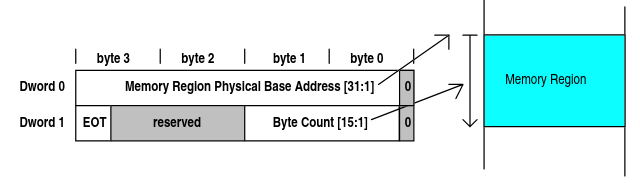
\includegraphics[scale=0.8]{../figures/prd.png}
		\end{center}
		Notiamo che le regioni indicate dall'indirizzo base dell'entrata PRD può essere al massimo di 64 KiB. Per questo lato hardware si può usare un sommatore a sole 16 cifre.
		In ogni caso, questo non sarà un problema in quanto vorremo trasferire buffer in memoria virtuale una pagina (4 KiB) alla volta.
\end{itemize}

A questo punto basterà definire i passaggi di un operazione di trasferimento:
\begin{enumerate}
	\item Si prepara una tabella PRD in memoria;
	\item Si carica l'indirizzo base della tabella PRD nel registro BMDTPR, quindi si ripuliscono i bit di interruzione ed errore del registro di stato BMSTR;
	\item Si fornisce il comando appropiato sul registro BMCMD;
	\item Si attiva il bit 0 del registro BMCMD per attivare il bus mastering;
	\item Il controllore DMA trasferisce i dati secondo quanto disposto finora;
	\item Alla fine della trasmissione il controllore segnala la fine dell'operazione su una linea di interruzinoe;
	\item In risposta all'interruzione, si resetta il bit 0 del registro BMCMD, e si legge lo stato dal controllore e dal disco per capire se l'operazione è andata a buon fine.
\end{enumerate}

\subsubsection{Controller IDE su bus PCI}
Per l'inserzione di un controllore di questo tipo in un bus PCI dobbiamo renderci conto di alcuni dettagli:
Nei registri dello spazio di configurazione del dispositivo si devono attivare dei flag particolari per segnalare la possibilità che questo lavori in bus mastering.

\subsubsection{Controller IDE nel kernel}
Vediamo infine come il controllore DMA dell'hard disk ATA viene gestito nel kernel.
La libreria \lstinline|libce| definisce i registri del controllore:
\begin{lstlisting}[language=C++, style=codestyle]	
namespace bm {
	extern ioaddr iBMCMD; // Bus Master Command
	extern ioaddr iBMSTR; // Bus Master Status Register
	extern ioaddr iBMDTPR; // Bus Master Descriptor Table Pointer
}
\end{lstlisting}
e le relative funzioni per l'inizializzazione, l'acknowledge, ecc...

L'unica interfaccia ATA montata nel sistema è quindi descritta dal descrittore:
\begin{lstlisting}[language=C++, style=codestyle]	
// descrittore di interfaccia ATA
struct des_ata {
	// Ultimo comando inviato all'interfaccia
	natb comando;
	// Indice di un semaforo di mutua esclusione
	natl mutex;
	// Indice di un semaforo di sincronizzazione
	natl sincr;
	// Quanti settori resta da leggere o scrivere
	natb cont;
	// Da dove leggere/dove scrivere il prossimo settore
	natb* punt;
	// Array dei descrittori per il Bus Mastering
	natl* prd;
};
\end{lstlisting}
che tiene conto dell'operazione corrente.

A questo punto il processo esterno dedicato all'hard disk dovrà limitarsi ad inviare i comandi corretti seguendo la scaletta appena riportata.
Unica parte di interesse è quella della preparazione della tabella PRD, per cui bisogna tenere conto che il controllore DMA necessita di indirizzi fisici, e che legge sequenzialmente a partire da tali indirizzi fisici (perciò non si possono superare i 4 KiB della dimensione di pagina).
Per fare questo, e tenere conto di buffer in memoria che iniziano potenzialmente a metà pagina, si sfrutta la funzione \lstinline|prepare_prd()|:
\begin{lstlisting}[language=C++, style=codestyle]	
bool prepare_prd(des_ata *d, natb* vett, natb quanti)
{
	natq n = quanti * DIM_BLOCK;
	int i = 0;

	while (n && i < MAX_PRD) {
		paddr p = trasforma(vett);
		natq  r = DIM_PAGINA - (p % DIM_PAGINA);
		if (r > n)
			r = n;
		d->prd[i] = p;
		d->prd[i + 1] = r;

		n -= r;
		vett += r;
		i += 2;
	}
	if (n)
		return false;
	// il bit end of table
	d->prd[i - 1] |= 0x80000000;
	return true;
}
\end{lstlisting}

A questo punto si possono fornire all'utente primitive per l'accesso all'hard disk sia a controllo interruzione (come avevamo già visto, implementato in \lstinline|libce|) sia in DMA.
Queste saranno:
\begin{itemize}
	\item \textbf{Controllo interruzione:} vediamo ad esempio l'operazione di ingresso.
\begin{lstlisting}[language=C++, style=codestyle]	
// fondamentalmente un wrapper per hd::start_cmd di libce, che aggiorna il descrittore
void starthd_in(des_ata* d, natb vetti[], natl primo, natb quanti)
{
	d->cont = quanti;
	d->punt = vetti;
	d->comando = hd::READ_SECT;
	hd::start_cmd(primo, quanti, hd::READ_SECT);
}

// la primitiva vera e propria
extern "C" void c_readhd_n(natb vetti[], natl primo, natb quanti)
{
	des_ata* d = &hard_disk;

	// controlli (c_access)

	sem_wait(d->mutex);
	starthd_in(d, vetti, primo, quanti);
	sem_wait(d->sincr);
	sem_signal(d->mutex);
}
\end{lstlisting}
\item \textbf{DMA:} vediamo sempre l'operazione di ingresso:
\begin{lstlisting}[language=C++, style=codestyle]	
void dmastarthd_in(des_ata* d, natb vetti[], natl primo, natb quanti)
{
	// passo 1 della scaletta
	if (!prepare_prd(d, vetti, quanti)) {
		flog(LOG_ERR, "dmastarthd_in: numero di PRD insufficiente");
		sem_signal(d->sincr);
		return;
	}

	d->comando = hd::READ_DMA;
	d->cont = 1;

	// passo 2
	paddr prd = trasforma(d->prd);
	bm::prepare(prd, false);
	
	// passo 3
	hd::start_cmd(primo, quanti, hd::READ_DMA);
	bm::start();
}
\end{lstlisting}
\end{itemize}

A operazioni terminate, il processo esterno dovrà chiaramente interpretare correttamente le interruzoni che riceve in base al tipo di comando dato:
\begin{lstlisting}[language=C++, style=codestyle]	
void estern_hd(natq)
{
	des_ata* d = &hard_disk;
	for(;;) {
		d->cont--;
		hd::ack();
		switch (d->comando) {
		// questi sono i casi gia visti
		case hd::READ_SECT:
			hd::input_sect(d->punt);
			d->punt += DIM_BLOCK;
			break;
		case hd::WRITE_SECT:
			if (d->cont != 0) {
				hd::output_sect(d->punt);
				d->punt += DIM_BLOCK;
			}
			break;
		case hd::READ_DMA:
		case hd::WRITE_DMA:
			// qui si fa l'acknowledge, passo 7 della scaletta
			bm::ack();
			break;
		}
		if (d->cont == 0)
			sem_signal(d->sincr);
		wfi();
	}
}
\end{lstlisting}

\end{document}
